%======================================================================
% To compile this file you have to set the .tex file path:
% setenv TEXINPUTS .:${PWD}/../../../::
%
% Use latex or pdflatex to compile.
%
% Author: C.Leonidopoulos, E. Meschi (parts stolen from N. Amapane)
% $Date: 2007/03/21 12:36:59 $  $Revision: 1.11 $
%
%======================================================================
\documentclass[a4paper]{cmspaper}
\usepackage{lineno} % line numbering for draft
\usepackage{ifthen}

%======================================================================
% Check for PDFLaTeX/LaTeX 

\newif\ifpdf
\ifx\pdfoutput\undefined
\pdffalse 
\else
\pdfoutput=1 
\pdftrue
\fi

\ifpdf  % ============== we are running PDFLaTeX
\usepackage{color}
\usepackage[pdftex]{graphicx,graphics}
\usepackage{epsfig}
\usepackage{pdflscape}
\usepackage[bookmarksnumbered,bookmarksopen,bookmarksopenlevel=1,
              colorlinks,
              linkcolor=blue,                      
              citecolor=blue, 
              urlcolor=blue]{hyperref}                                 
\pdfinfo{
  /Title  (DQM Project Document)
  /Author (...)
  /Keywords (DQM, Online, DAQ, CMS)
  }

\DeclareGraphicsExtensions{.pdf}

\else   % ============== we are not running PDFLaTeX
\usepackage{epsfig}
\usepackage{lscape}

\DeclareGraphicsExtensions{.eps}

%fake pdflatex commands.
\newcommand{\pdfbookmark}[3][1]{}
\newcommand{\href}[2]{#2}

\fi

%==============================================================================

\newcommand {\ie}{\mbox{\sl i.e. }}     %i.e.
\newcommand {\eg}{\mbox{\sl e.g. }}     %e.g.

\begin{document}

%==============================================================================
% title page for few authors

\begin{titlepage}

% select one of the following and type in the proper number:
%   \cmsnote{2005/000}
%  \cmsnote{2007/XYZ}
%  \conferencereport{2005/000}
   \date{\today}
\smallskip
\smallskip
\rightline{\bf Version 0.1}

\vspace{1cm}

\title{DQM Group Project Document\\[0.5cm]
\normalsize }

\vspace{1cm}

  \begin{Authlist}
%     Authors
%       \Instfoot{Institut}{Institut}
    G.\,Della Ricca, A.\,Meyer, A.\,Rizzi, I.\,Segoni, L.\,Tuura
    
  \end{Authlist}

% if needed, use the following:
%\collaboration{Flying Saucers Investigation Group}
%\collaboration{CMS collaboration}

\vspace{1cm}

  \begin{abstract}
    \pdfbookmark[1]{Abstract}{Abstract}
    The note describes the baseline central CMS Data Quality Monitoring 
    and Data Certification System. Tasks for development, commissioning and 
    operation of DQM services are listed.
  \end{abstract} 

% if needed, use the following:
%\conference{Presented at {\it Physics Rumours}, Coconut Island, April 1, 2005}
%\submitted{Submitted to {\it Physics Rumours}}
%\note{Preliminary version}
  
\end{titlepage}

\thispagestyle{empty}
\tableofcontents

\newpage

\setcounter{page}{1}%JPP
%\linenumbers
%===============================================================================================

\section{Introduction} 
\label{sec:introduction}

Data Quality Monitoring is critically important for the detector and operation efficiency
and for the reliable certification of the recorded data for physics analyses. 
The CMS end-to-end DQM chain comprises
\begin{itemize}
\item live online detector and trigger monitoring (section \ref{sec:online})
\item offline reconstruction monitoring (section \ref{sec:offline})
\item data certification of events and datasets for physics analysis (section
\ref{sec:certification})
\item the visualization of the monitoring results (\ref{sec:gui}).
\end{itemize}

The CMS DQM software framework provides tools for the creation, filling, transport, archival and visualization of histograms. The software includes standardized algorithms to perform automated quality and validity tests on the DQM distributions. 
DQM processes are operating on the online data in P5 as well as during offline processing at the Tier-0, 1, 2 centers. 
In addition the DQM system is in use or will be used for other purposes, such as
\begin{itemize}
\item the monitoring of calibration processing and the validation of the calibration results
\item the validation of software releases
\item the monitoring of the DAQ hardware status and data throughput
\item the retrieval of DQM-relevant quantities from the conditions database
\end{itemize}
Use of DQM tools is also foreseen for the interactive and semi-automated processing of data at the CAF. 

\section{The CMS-wide DQM Group} 
\label{sec:charge}

A CMS-wide DQM group has been created with the aim to realize the above described goals 
in an efficient and standardized way for all CMS. The group carries the following charge.

\subsection{Charge to the DQM Group}
Data Quality Monitoring appears in various places across the experiment.
The charge of the DQM Groups is as follows:
\begin{itemize}
\item   identify the places, and construct the end-to-end connected chain, where DQM is done
\item   coordinate the technical implementation, including the software architecture and the service deployment, and harmonize the code and procedures used in DQM across the experiment
\item  identify and make widely available the most important plots and features to assure that data being taken and being analysed are of good quality
\item   identify the different timescales (or Dt) for reporting of DQM information required at the places identified in the above-mentioned connected end-to-end chain
\item  evaluate health of runs and identify "good runs". Moreover, tag each event with the appropriate detector conditions to indicate which detector information can be used.
\end{itemize}

\paragraph{Composition of the DQM Group}
The Group will be convened by two physicists (I. Segoni, A. Meyer) and a technical coordinator (L.
Tuura).
One DQM expert from each of the sub-detector DPGs (Tracker, ECAL, HCAL, Muons(2), Level-1 Trigger, DAQ) and areas (HLT, Commissioning and Run, Offline and Physics) will be assigned.

%CHECK need alca here

\paragraph{Reporting}
The DQM conveners will report via the Commissioning and Run Coordinator and the Spokesperson to MP3

\paragraph{Timeline}
First report in May, interim report in CMS Week in June, first deployment during the CRAFT after Cyprus Week.


\subsection{Near future Goals and Priorities}

Given the above charges the near future priorities must be to finish the
development, implementation and deployment of the complete code base for the end-to-end system
and to establish and consolidate the DQM system operation with minimal maintenance needs. 

% Introduction
%===============================================================================================
%===============================================================================================
%===============================================================================================
% Online 

\section{The Online DQM System}
\label{sec:online}

Online DQM applications are operated on the cms-cluster at P5 on event data. 
DQM distributions are created at two different levels:

\begin{enumerate}
\item {\bf DQM Sources in the HLT Filter Units:} \\
A limited number of histograms, as implemented in analyzer modules, can be processed at the level of the HLT where events are available at a rate of up to 100 kHz. The histograms (as stored in monitoring elements (ME)) are shipped out from the HLT filter units to the Storage Managers at the end of each luminosity section. Identical histograms from different filter units are summed up and sent to the SMProxyServer, a single access point, which provides access to the ME through a DQM histogram server to consumer applications. The SMProxyServer also saves the DQM histograms to files. 
\item {\bf DQM Sources operating off the Storage Manager Event Server:} \\
The Storage Manager Proxy Server also provides an event server which delivers events at the rate of order 10-15 Hz to event consumer applications. The events available events are part of special DQM stream the contents and selection are specified by the DQM group as part of the HLT configuration. 
\end{enumerate}
The storagemanager system is sketched in Fig.~\ref{fig:sm}.

\begin{figure}[!htbp]
\begin{center}
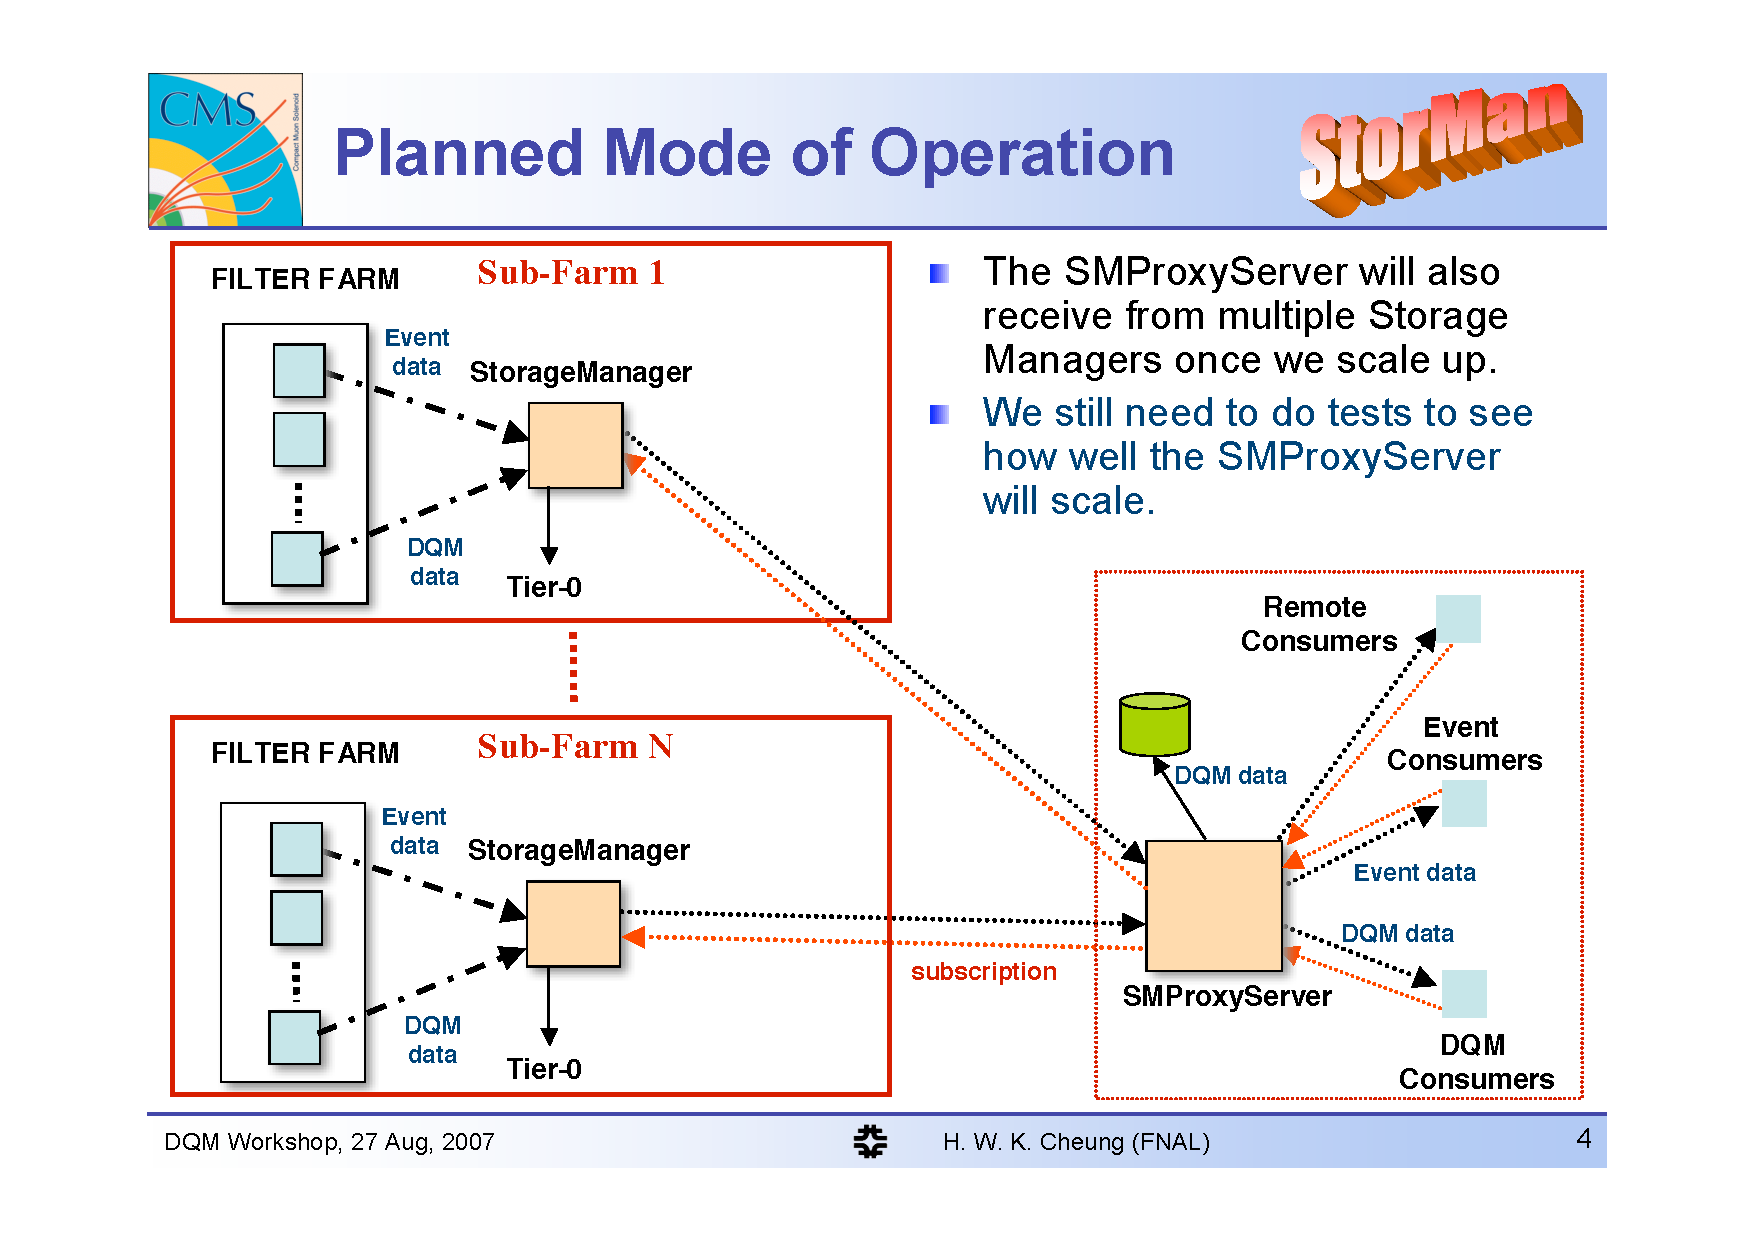
\includegraphics[width=0.9\textwidth]{SM}
\caption{Storage Manager Event and DQM-ME Server 
(figure taken from \cite{talk:harry}).}
\end{center}
\label{fig:sm}
\end{figure}

Fig.~\ref{fig:overview} shows a sketch of the baseline design of the architecture for data quality monitoring using events served by the Storage Manager event server. Several DQM source-client processes (typically one per subsystem) retrieve events through http-request from the event server. The ME (including environmental information, e.g. the runnumber, as well as reference histograms and results from quality tests) are served to one central DQM GUI for visualisation. Alarm states, based on quality test results are also served to the same central display.

\begin{figure}[!htbp]
\begin{center}
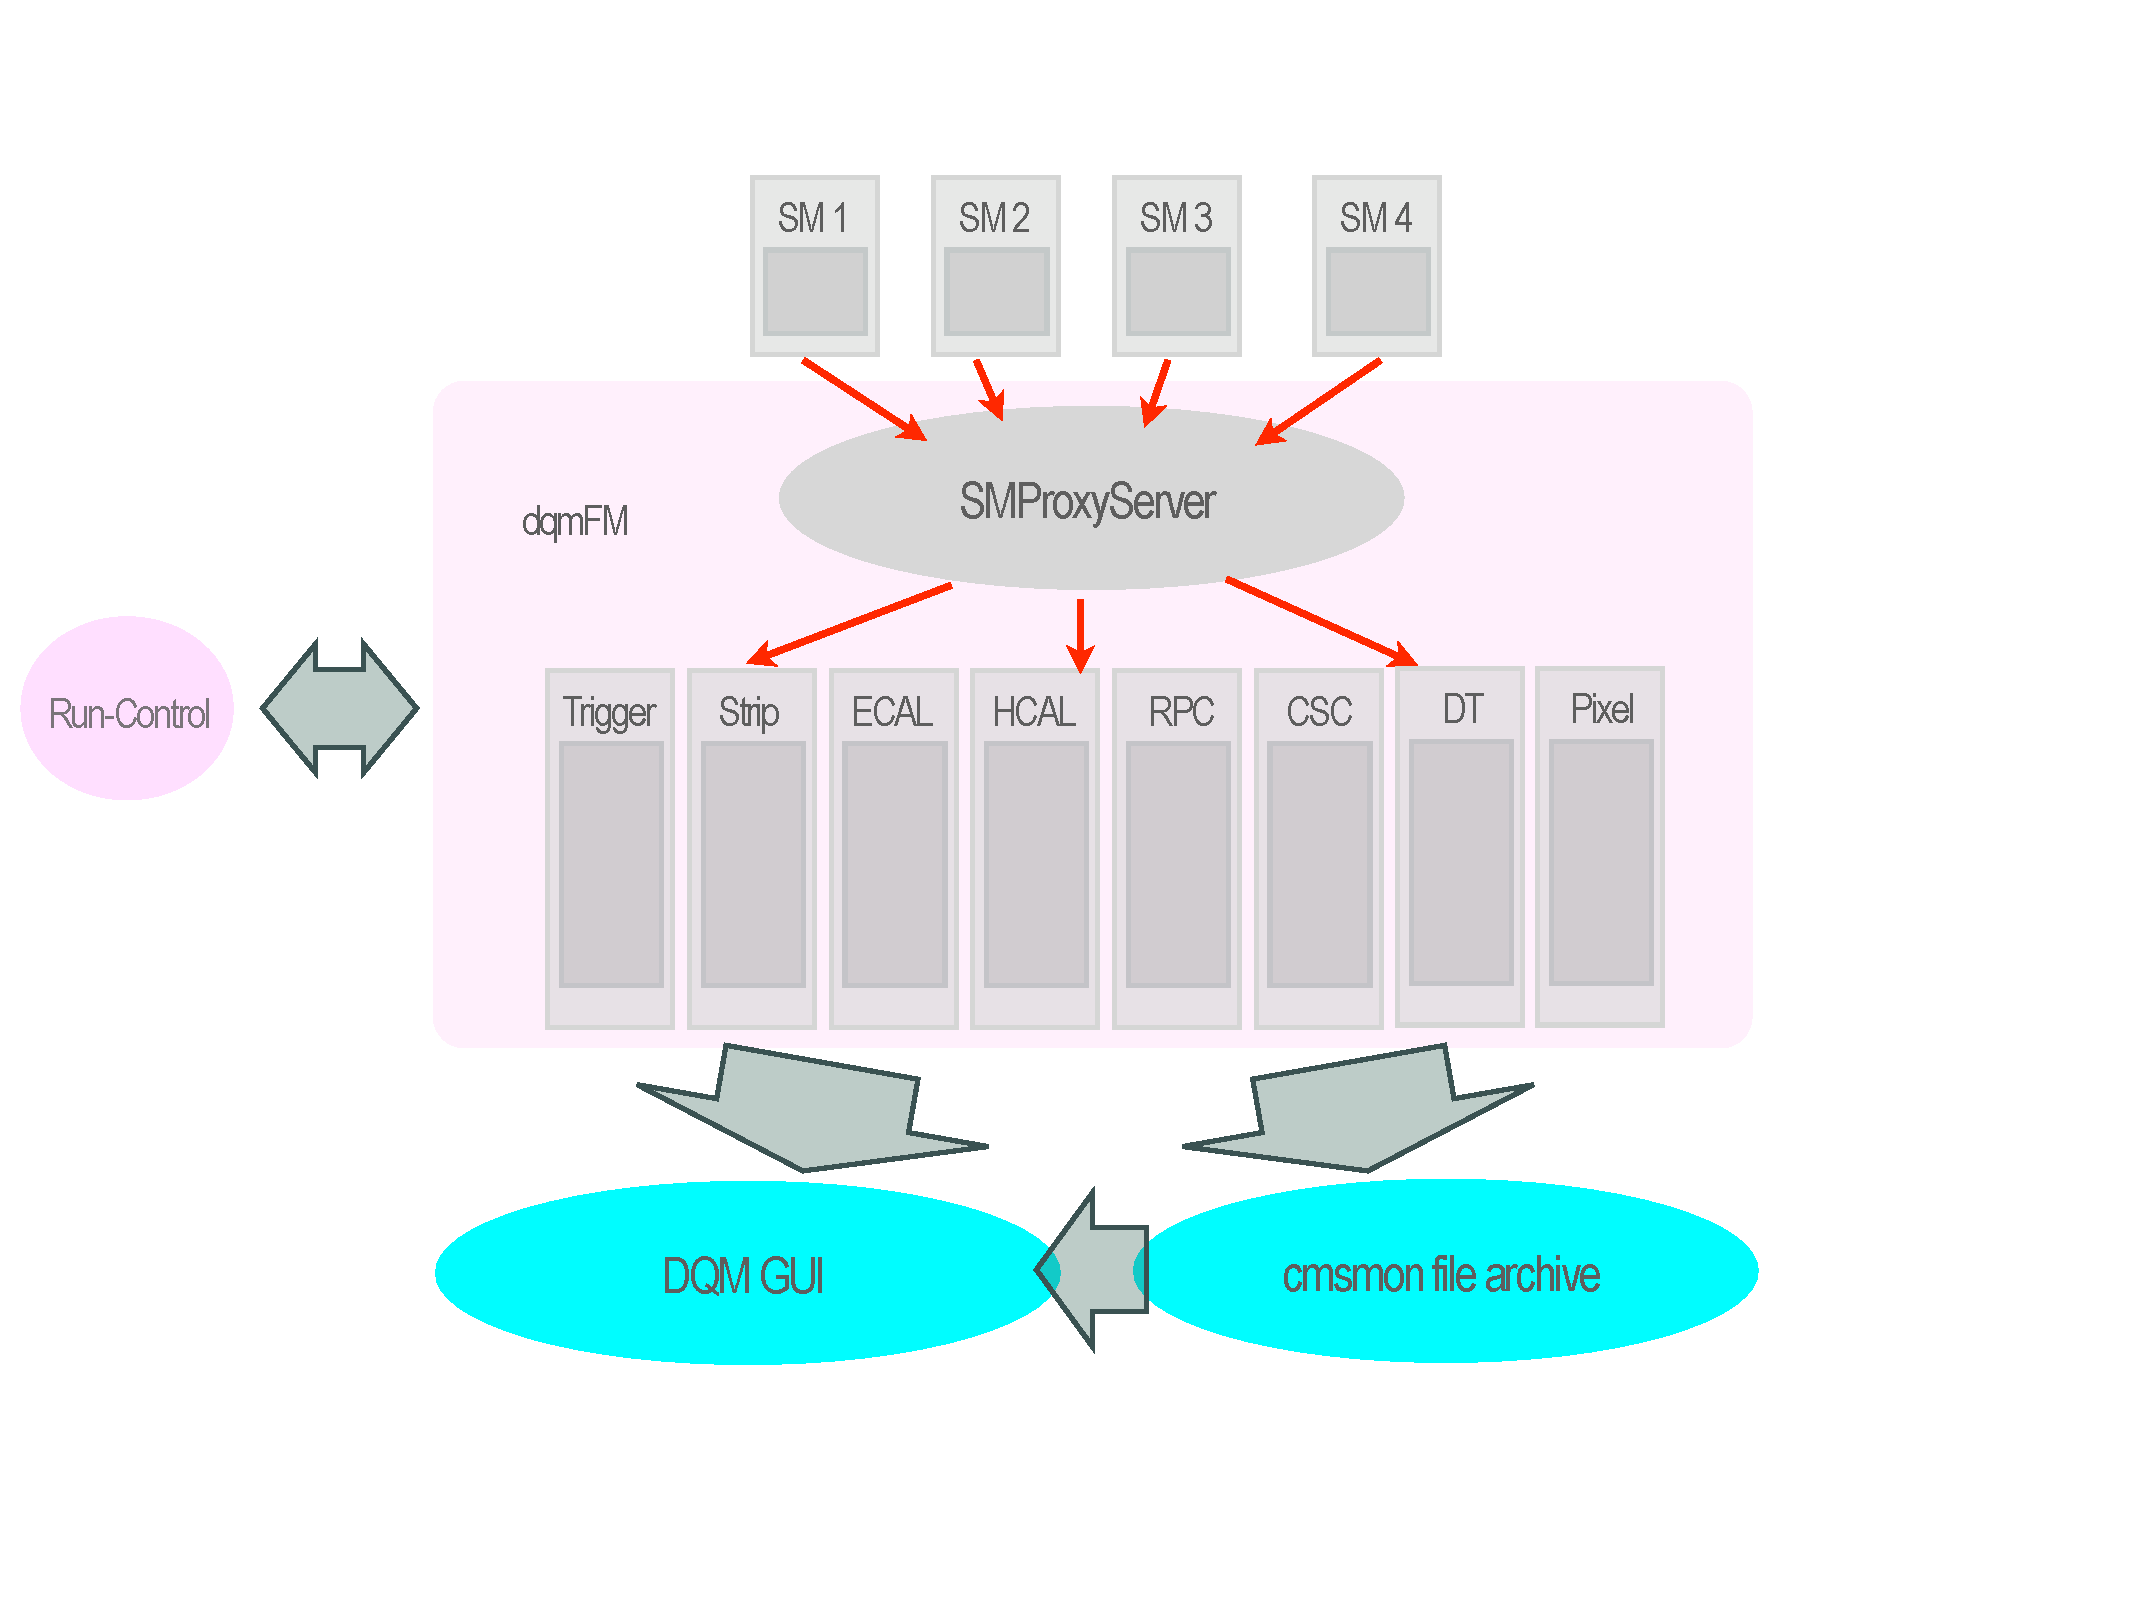
\includegraphics[width=0.9\textwidth]{dqm_online}
\caption{Sketch of the baseline online DQM system.}
\end{center}
\label{fig:overview}
\end{figure}


\subsection{Online DQM Applications}

Event consumer applications are operated on the DQM stream and select events based on trigger paths. The SMProxyServer baseline design foresees no special handling or sorting of events. There will be no provision for parallel event consumers to receive always different events.
DQM applications implement EDAnalyzers for histogram creation and filling. The histograms are stored as MonitorElements and registered to the DQMStore service. Qualitytests are accessible through a generic Qualitytests module and configurable through xml. The specification and implementation of the algorithms is responsibility of the detector performance groups. The DPG provide configurations to the DQM group for review. Reviewed configurations are included in central DQM operation.
The DQM online processes, i.e. the SMProxyServer and the DQM applications (as well as the eventdisplay) are operated within the CMS run-control framework using the level-one DQM function manager. The DQM GUI webservers are operated separately, outside the run-control system

\subsection{Online DQM Stream HLT Configuration}

The event server will be bound to one particular output module that provides the DQM stream.
The DQM stream is a transient event stream that is configurable on the HLT side where the DQM group will be able to specify what HLT paths are to be output and maybe additional paths of their choice, within the general HLT constraint.
Consumer applications can select among the paths which are selected by the DQM output module.

The baseline for the DQMStream contents (i.e. products) is to provide
just raw-data, and to re-run the reconstructions (as much as necessary)
at the DQM consumer level. Additional HLT information can be provided
on request by the consumer application responsible. Optimization of 
event contents, paths and rate sharing is done based on prioritization 
of overall monitoring requirements and bandwidth limitations.
Authoritative priority and optimization decisions are taken based on
discussions within the CMS-wide DQM group.

\subsection{Online DQM Output Archiving and Retrieval}

Each source-client process produces root-file output initially once per run, at the end of a run. 
The root-files are archived in a disk-based spool-area cmsmon.cern.ch.
Several root-files are concatenated into large files. These large
files are made accessible on the web through the DQM webserver-based 
GUI (section \ref{sec:gui}) and backed up to tape. The file handling,
merging, archival, registration with the webserver and backup to tape
are handled by scripts that are operated from cmsmon.
Specific files in the spool-area can be tagged for the purpose of 
providing reference histograms. 

%==========================================================
% this subsection is common to all sections, please fill in
\subsection{Online DQM Integration and Operation}

\subsubsection*{Integration}

The main orientation of the integration work is the standardization of the DQM processes, i.e. the definition and enforcement of standardized DQM interfaces 
and naming conventions.
A large amount of work is spent supporting and consulting the
subsystem responsibles as well as persons starting to use
DQM tools.

\subsubsection*{Operation}

A skeleton online DQM system has been in operation at P5 since November.
Production-level operation was achieved for a few days in a row during
the global runs. This was made possible through maintenance efforts that would be unsustainable over a larger period of time.
At present the development, deployment and maintenance of the 
online production system requires 1-2 FTE. With additional help 
integration and deployment could be accelerated significantly.
Once production is fully established the amount of work for 
operation and maintenance of the online DQM system is estimated to be at least 
1 FTE.


%===============================================================================================
%===============================================================================================
%===============================================================================================
% Offline 
\section{The Offline DQM System}
\label{sec:offline}

\begin{figure}[!htbp]
\begin{center}
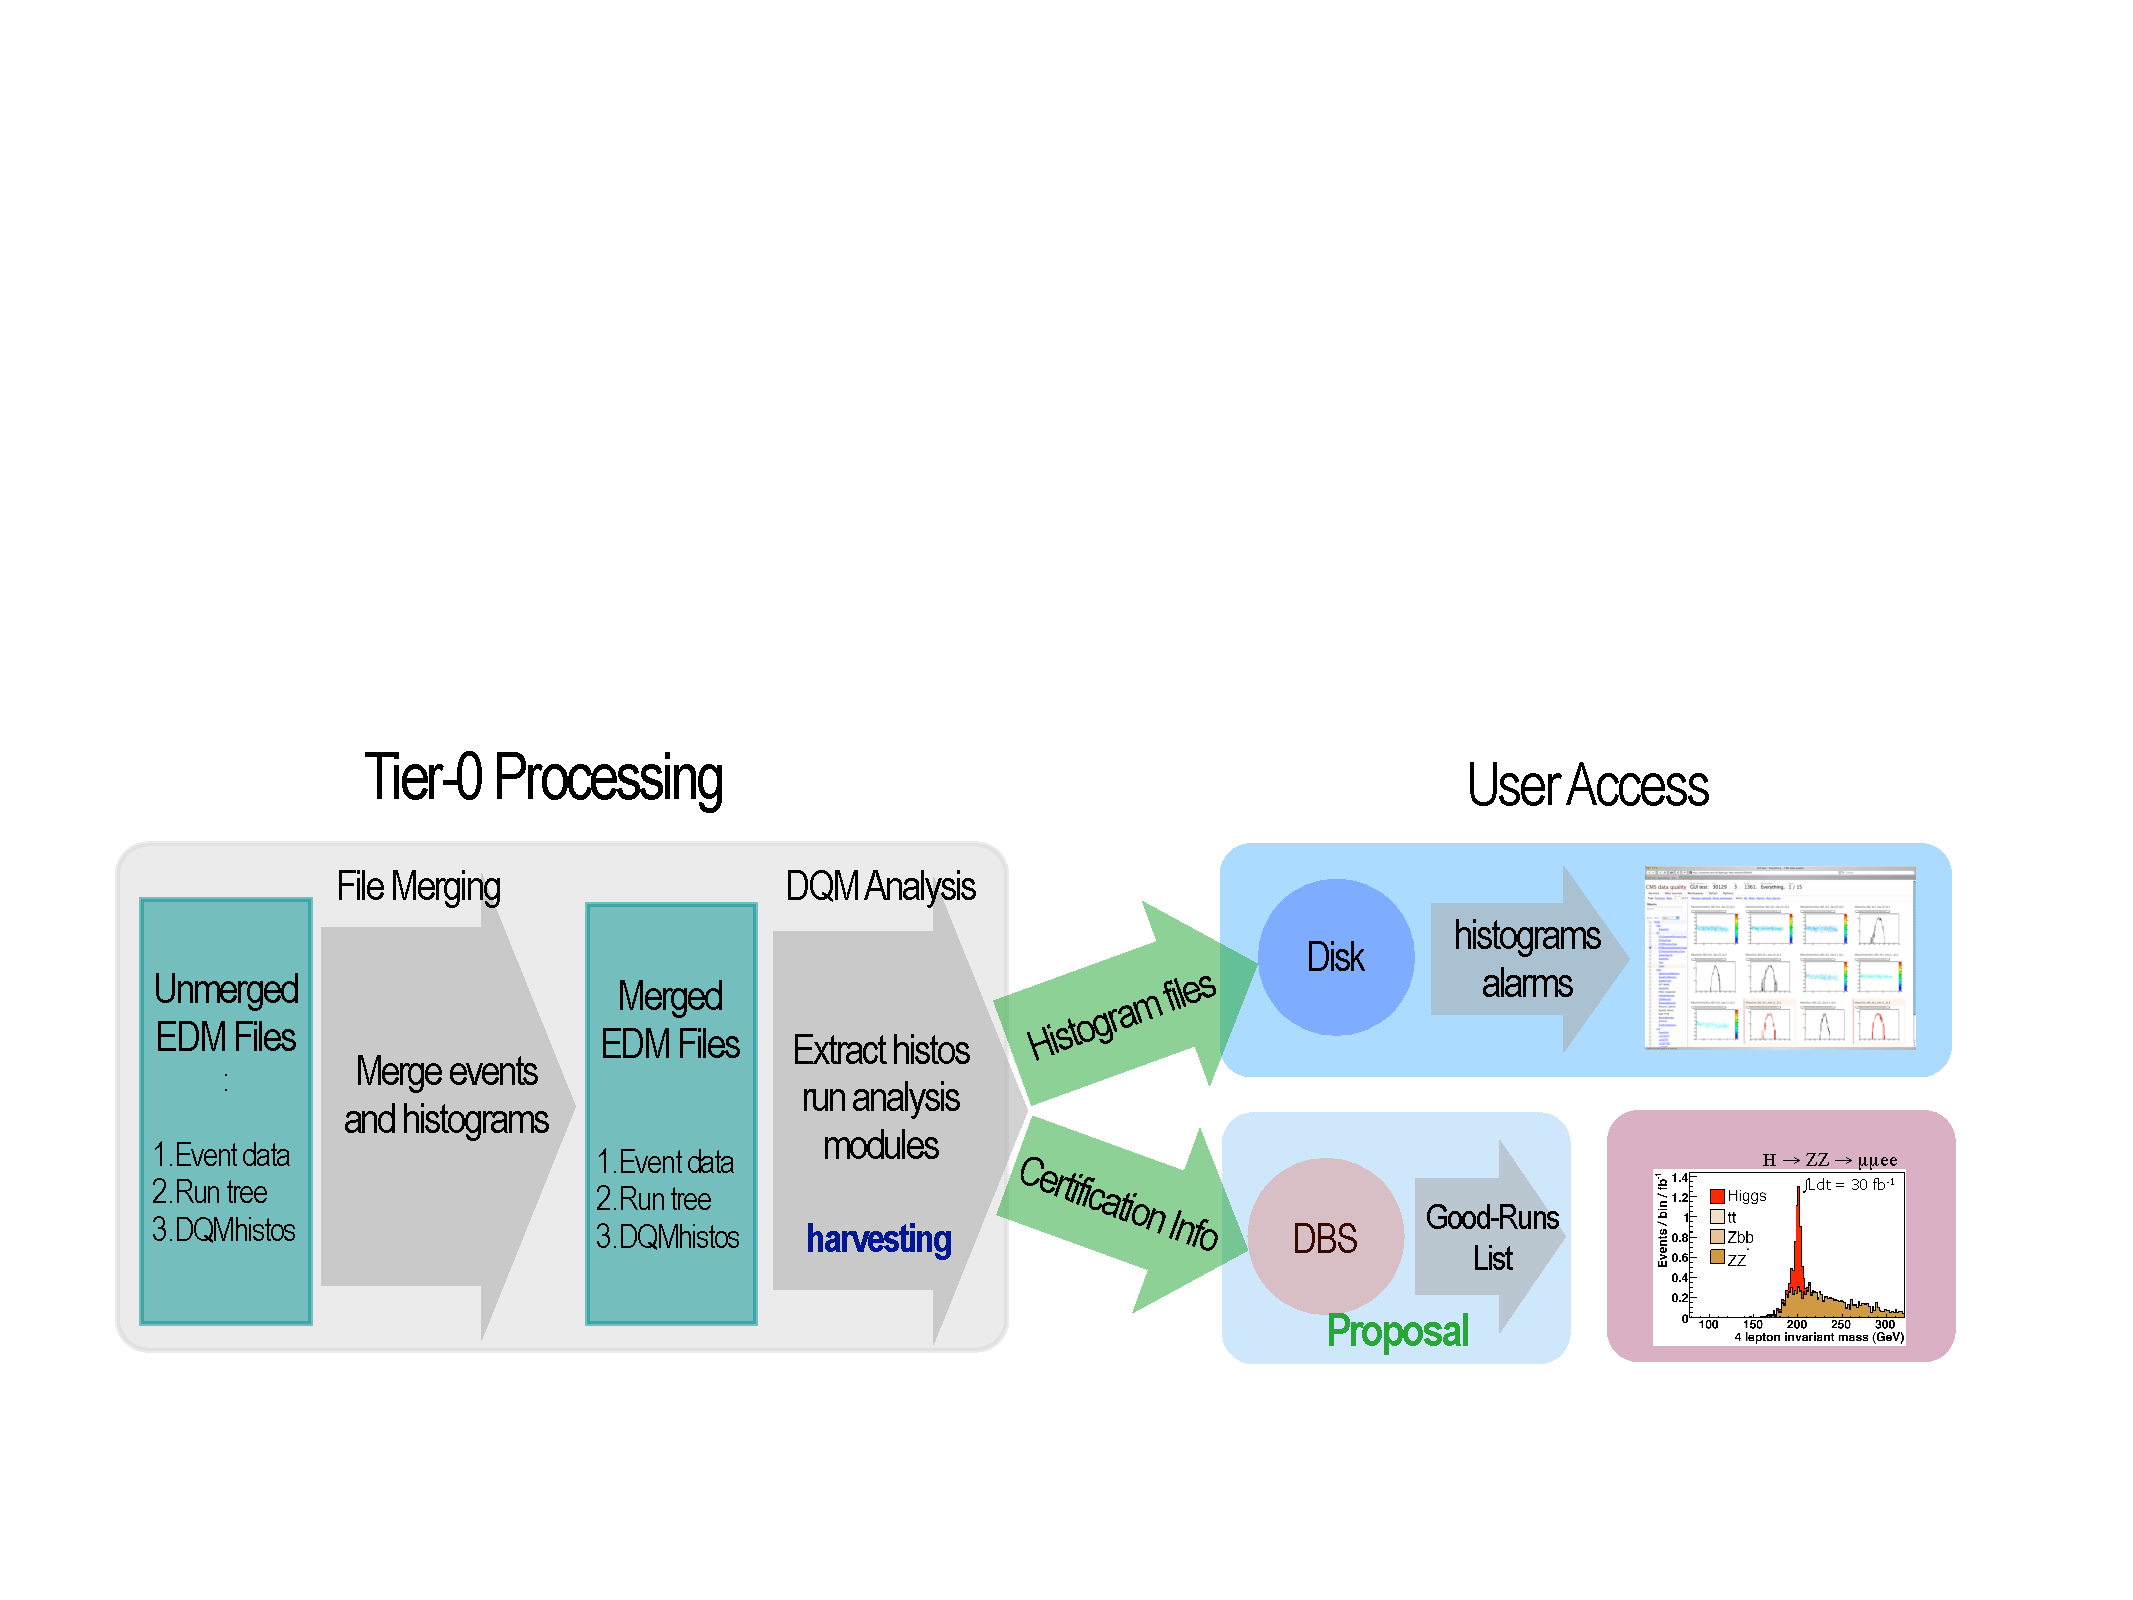
\includegraphics[width=0.9\textwidth]{dqm_tier0}
\caption{DQM data flow at Tier-0}
\end{center}
\label{fig:dqmoffline}
\end{figure}


\subsection{Prompt Reconstruction Monitoring}


Tier-0 DQM processing consists of two steps. In the first step
the histograms are created, filled with event information and stored 
in the EDM job output files (along with the processed events).
In a second step, the histograms are extracted from the EDM files.
They are merged (summed) together, and analysis and
quality test steps are performed. The second step includes
the calculation of physics data certification decisions.

At the end of the second step the output histograms are stored in files 
which are transfered to the file archive on the histogram DQM GUI server machine
and the certification information is written to the conditions database and into DBS.

\subsubsection{Histogram creation and filling}

% here put some details about:
DQM histograms creation, filling, storage in EDM files 
and subsequent summation of histograms during EDM file merge.
            + Tier-0, DQMOffline (package and sequence definitions), DPG, POG

\subsubsection{Harvesting step}

\begin{itemize}
\item{Extraction and Quality testing}

\item{Physics Data Certification} 

refer to section \ref{sec:certification})


\end{itemize}

\subsection{Release Validation}

\subsection{Calibration Monitoring}

\begin{figure}[!htbp]
\begin{center}
%\includegraphics[width=0.9\textwidth]{dqm_alca}
\caption{Envisaged DQM data flow for calibration and alignment purposes.}
\end{center}
\label{fig:dqmalca}
\end{figure}

Calibration workflow layout and integration (mostly CAF)

\subsection{DQM at the CAF}
\label{sec:caf}

Define support of CAF activity by DQM group.
Handshake between root-file output and offline DQM GUI

%==========================================================
% this subsection is common to all sections, please fill in 
\subsection{Offline DQM Integration and Operation}

\subsubsection*{Integration}

\subsubsection*{Operation}


% Offline 
%===============================================================================================
%===============================================================================================
%===============================================================================================
% Certification 
\section{The Data Certification System}
\label{sec:certification}

In the certification system detector hardware state information is combined with results 
from DQM quality tests providing certification bits for event selection in physics analyses.
The data certification system is part of the offline DQM processing at Tier-0 
(and Tier-1 for reprocessings). The following proposal for a data certification workflow and persistency has been circulated. This proposal concerns decisions for
\begin{itemize}
\item the retrieval and calculation of certification information (section \ref{sec:cert:calc})
\item the persistent storage of this information (section \ref{sec:cert:schema})
\item necessary steps for the commissioning of a baseline system (section \ref{sec:cert:plan})
\end{itemize}

%Reference to wiki pages
  
\subsection{Retrieval and calculation of certification information}
\label{sec:cert:calc}

Certification algorithms will be run as part of the DQM histogram harvesting and analysis step (2nd step). The certification decisions will be determined per luminosity section based on input from
\begin{itemize}
\item DCS  HV
\item RunInfo DAQ/RCMS
\item DQM online
\item DQM offline.
\end{itemize}
        
The relevant conditions information from DCS, RCMS and DQM online are stored in Orcoff and can be retrieved from there. Appropriate certificiation algorithms to combine these inputs will  be provided by the DPG. 

The granularity should be detector segments, i.e. appropriate fractions of subdetectors, e.g. for Tracker the segmentation could be TIB, TOB, TID, TEC, PXB, PXF (see page 3 of \cite{datacert:gutsche}). For each of the segments a number of inputs will be filled, namely DCS, DAQ, online DQM, offline DQM (and potentially Power and Cooling, as indicated at bottom of page 4 of \cite{datacert:gutsche}).
The certification algorithms yield floating point numbers for each detector segment, representing the working fraction of the respective detector segment.
   
For each detector segment appropriate thresholds are defined such that binary decisions, status bits "good" or "bad", can be obtained from the floating point numbers. In case no number was calculated
the decision bit "unknown" is set.

\subsection{Certification data storage schema}
\label{sec:cert:schema}

The floating point numbers as well as the detector status bits "good/bad/unknown" are stored in the conditions database (Orcoff) and in DBS for  each detector segment.

The schema in DBS and in Orcoff are identical.

The present DBS schema has been explained in \cite{datacert:gutsche}. The global and detailed information to be stored is sketched on page 8  of \cite{datacert:gutsche} for the example of tracker and TIB. 

\subsection{Development and Commissioning}
\label{sec:cert:plan}

As a first step, in order to gain experience, a python-script will be provided, which allows to manually set DQM-online quality global and detailed bits for each detector and detector segment. This script will be ready for use during CR0T and the online-DQM shift person in P5 will be in charge of filling it. The information will be in units of runs, not luminosity sections.

% Further steps
% It will be important to combine the knowledge of the DPG about possible detector failures
% with physics analysis requirements 
% i.e. synergy between POG/PAG and DPG.

%==========================================================
% this subsection is common to all sections, please fill in
\subsection{Data Certification System  Integration and Operation}

\subsubsection*{Integration}
\subsubsection*{Operation}


% Certification
%===============================================================================================
%===============================================================================================
%===============================================================================================
% GUI
\section{The Graphical User Interface Webserver System}
\label{sec:gui}

A unified customizable DQM GUI for viewing of online and offline data from P5, from CERN and from remote is provided. The goal is to have a tool with common look-and-feel for online and offline DQM data. The GUI comprises all capabilities for shift and expert use. In its final form it will replace the existing expert GUIs with no effective loss of functionality.

A webserver-based technology was chosen in order to provide both online, CERN and remote access with no overhead for single users to install particular software.

The DQM GUI comprises a webserver and a number of backends for access to online (live and from file), as well as offline DQM output (see fig.~\ref{fig:gui}). The webserver reuses web-tools technologies~\cite{webtools}. For the backend the Qt-independent parts of the previous iguana code are being reused~\cite{iguana}. The webservers for online-DQM are operated on the DQM worker nodes in the private network at P5. A reverse proxy-server on cmsmon.cern.ch provides world-wide user access. The webserver reads the histogram objects received from the backends, renders the histogram pictures as png pictures and provides navigation facilities. In the following the main requirements are listed~\cite{guimeeting,talk:lassi}.

\begin{figure}[!htbp]
\begin{center}
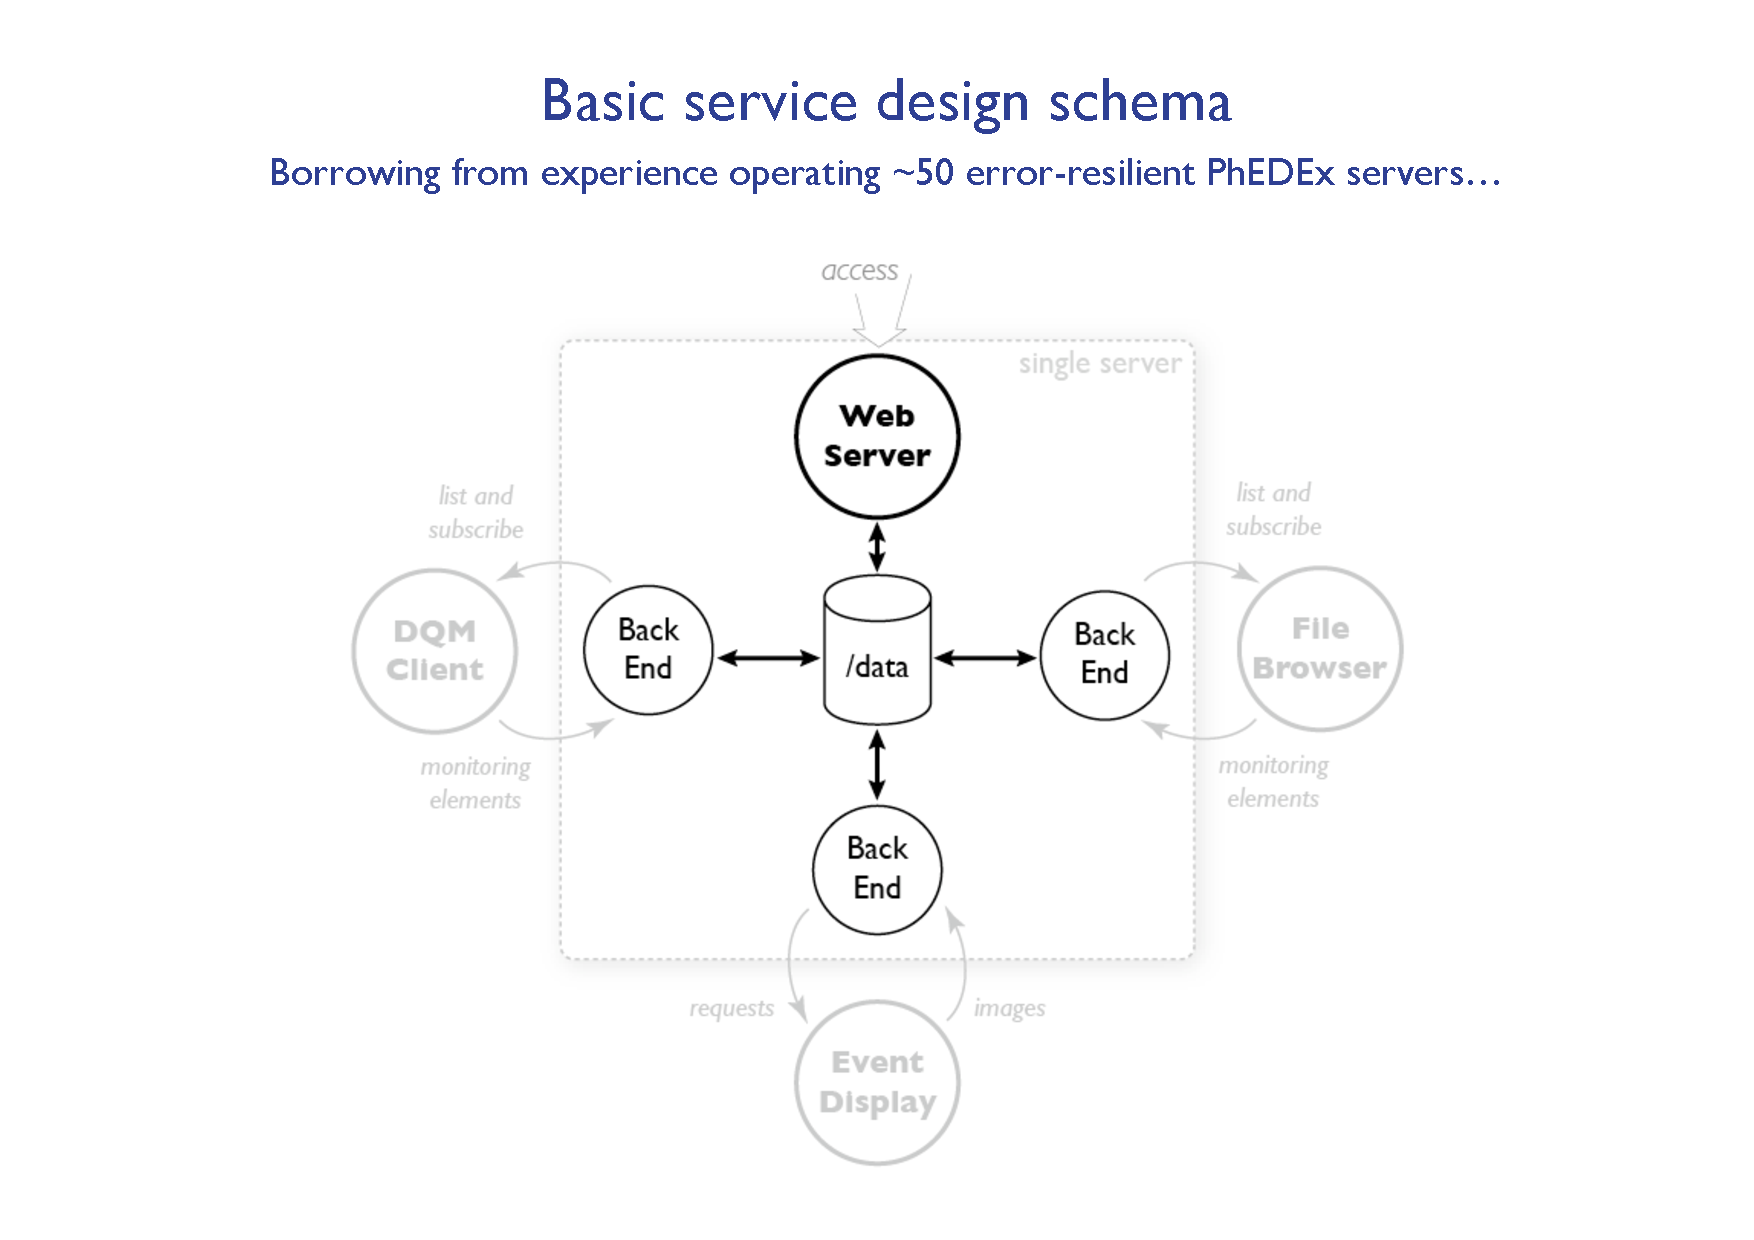
\includegraphics[width=0.9\textwidth]{GUI}
\caption{Webserver based DQM Visualization with different backend
for access to online DQM as well as output from offline processing
(figure taken from \cite{talk:lassi}). }
\end{center}
\label{fig:gui}
\end{figure}

\subsection{Requirements}

\begin{itemize}
\item Histogram collection, rendering and display
\begin{itemize}       
   \item The GUI collects DQM information from all possible sources, possibly including subsystem-based DQM facilities as well as results from XDAQ based DAQ monitoring. 
   \item Up to 12 histograms are displayed at once at any given time. 
   \item A summary display is provided that indicates available information, e.g. the current situation of subscriptions and histogram updates.
\end{itemize}
\item Histogram Navigation and Decoration 
\begin{itemize}
\item The same webserver GUI provides switches between different backends (e.g. live-online, online from file-archive, offline etc).
\item Operation modes, such as expert and shift, remote and P5, online and offline are configurable.
\item For online DQM a detector component based directory structure is used, reflecting the several subsystem-dependent sources.
\item A number of histogram views are foreseen, based on different aspects such as synoptic views (e.g. for shift operation), as well as detailed views based on geometrical position, frontend and cabling map, alarm state etc. In addition a search functionality (based on the histogram name is foreseen).
\item Individual layouts simplify retrieval of user-specified views making lengthy repetitive navigation obsolete. A slide show mode will be useful for the purpose of shift-browsing.
\item Subsystems can provide display plug-ins which specify the way histograms are rendered (colour-palettes and decorations etc.)
\item A facility for overlaying reference histograms is in place.
\item Customizable menus for histogram decoration (e.g. depending on quality test results) and labeling (including instructions to non-expert users (shift) about possible features that are significant of error states) are provided.
\item Facilities for histogram zooming and pointering are in place.
\item In order to display distributions of single LS a subtraction facility is foreseen, in which accumulated data from two subsequent LS are subtracted to retrieve the distributions of one single LS.
\item For navigation and interactivity aspects a webserver public interface is being considered. This way javascript components which conform with this interface can be collected in a library and attached to the GUI on demand.
\item Online DQM functionality beyond that implemented in iguana, e.g.\,components of the well-advanced implementation of DQM visualization tools based on XDAQ by the silicon and strip tracker groups is going to be realized. 
\item Visualization of live history and trends %CHECK
\item Full development, deployment of the error collector
and integration with offline data certification.
\item Assembly of static run-wise summary webpages (`page-1 of DQM')
\end{itemize}
\end{itemize}

\subsection{Online Summary Views}
\label{sec:summary}

The purpose of online DQM being prompt and efficient identification of problems, the most prominant goal of online Monitoring must be to distribute all relevant information quickly to where ever it is needed.

Each online DQM sub-system will provide three pieces of DQM summary information:
\begin{itemize}
\item the reportSummary ME (type: float) containing a global summary of the detector state
\item the reportSummaryMap ME (type: TH2F) containing a 2d histogram with report information as function of eta - phi.
\item the reportSummaryContents folder, containing a collection of MonitorElements of type float which are used to describe the behavior of sub-sub-system components. This collection of floats allows the sub-system to provide useful information about their inner/low-level state.
\end{itemize}
All three kinds of objects are under the sub-system responsibility, both booking and filling (the DQMEventInfo will be cleaned up).

This information is displayed in the following way:
\begin{itemize}
\item the EventInfo/reportSummary float ME will remain in the top table in the Summary workspace. this table is the only one shown by default.
\item by clicking on the 'sub-system' name in the table (in on/off fashion), the empty space below the table will show:
\begin{itemize}
\item on the left side the EventInfo/reportSummaryMap TH2D MEs
\item on the right side, a table (two columns, several rows) showing the list of the float MEs contained in EventInfo/reportSummaryContents, with their names and values (in the future we expect the names to change according to the sub-sytem needs, without changes in the GUI).
\end{itemize}
\end{itemize}

\subsection{Interactivity}

Interactivity is constrained to navigating through the list of available DQM results and visualizing them. In addition it is foreseen that users can modify the sensitivity of the display to alarm states by changing specific histogram decorations and sound-levels.

However, there will be no real-time interaction between the user (e.g. subsystem expert) and DQM-client applications. DQM applications can be configured to perform any activity required at the beginning of each run. In addition stand-alone DQM applications that receive events from the same Storage Manager event server can be launched at any time. 

%==========================================================
% this subsection is common to all sections, please fill in
\subsection{DQM GUI System Integration and Operation}

\subsubsection*{Integration}
\subsubsection*{Operation}


% GUI (Lassi)
%===============================================================================================
%===============================================================================================
%===============================================================================================
% Other systems

\section{DQM Interfaces To Other Systems}

\subsection{Database} 
\label{sec:database}

Automated and interactive DQM makes use of databases in various places. In particular
the DQM analyzers access the database through the standard CMSSW EventSetup interface.

Beyond that the main interest for DQM to use the database is for the purpose of
history and trend plotting. Quantities available in DQM client applications, such as summary quantities of histograms (e.g.\,means and widths of distributions) as well as the results from quality tests can be stored in the conditions database. Once in the database these conditions data produced by DQM clients can be correlated with non-event conditions data such as temperatures or DAQ monitoring information (trend-plots). Similarly history plots can be produced by plotting a given database-resident quantity versus time or runnumber.
A unified scheme of database usage for DQM purposes is being explored in cooperation between the subsystems and the database group.

In this context, the database group has proposed to re-use the DQM GUI for access 
to database information. 
The exactly requirements and needs are still to be worked out, based on input
from the subsystems, and the availability of qualified persons to work on the development and implementation of this interface needs to be confirmed, before a more detailed description can be given.

\begin{figure}[!htbp]
\begin{center}
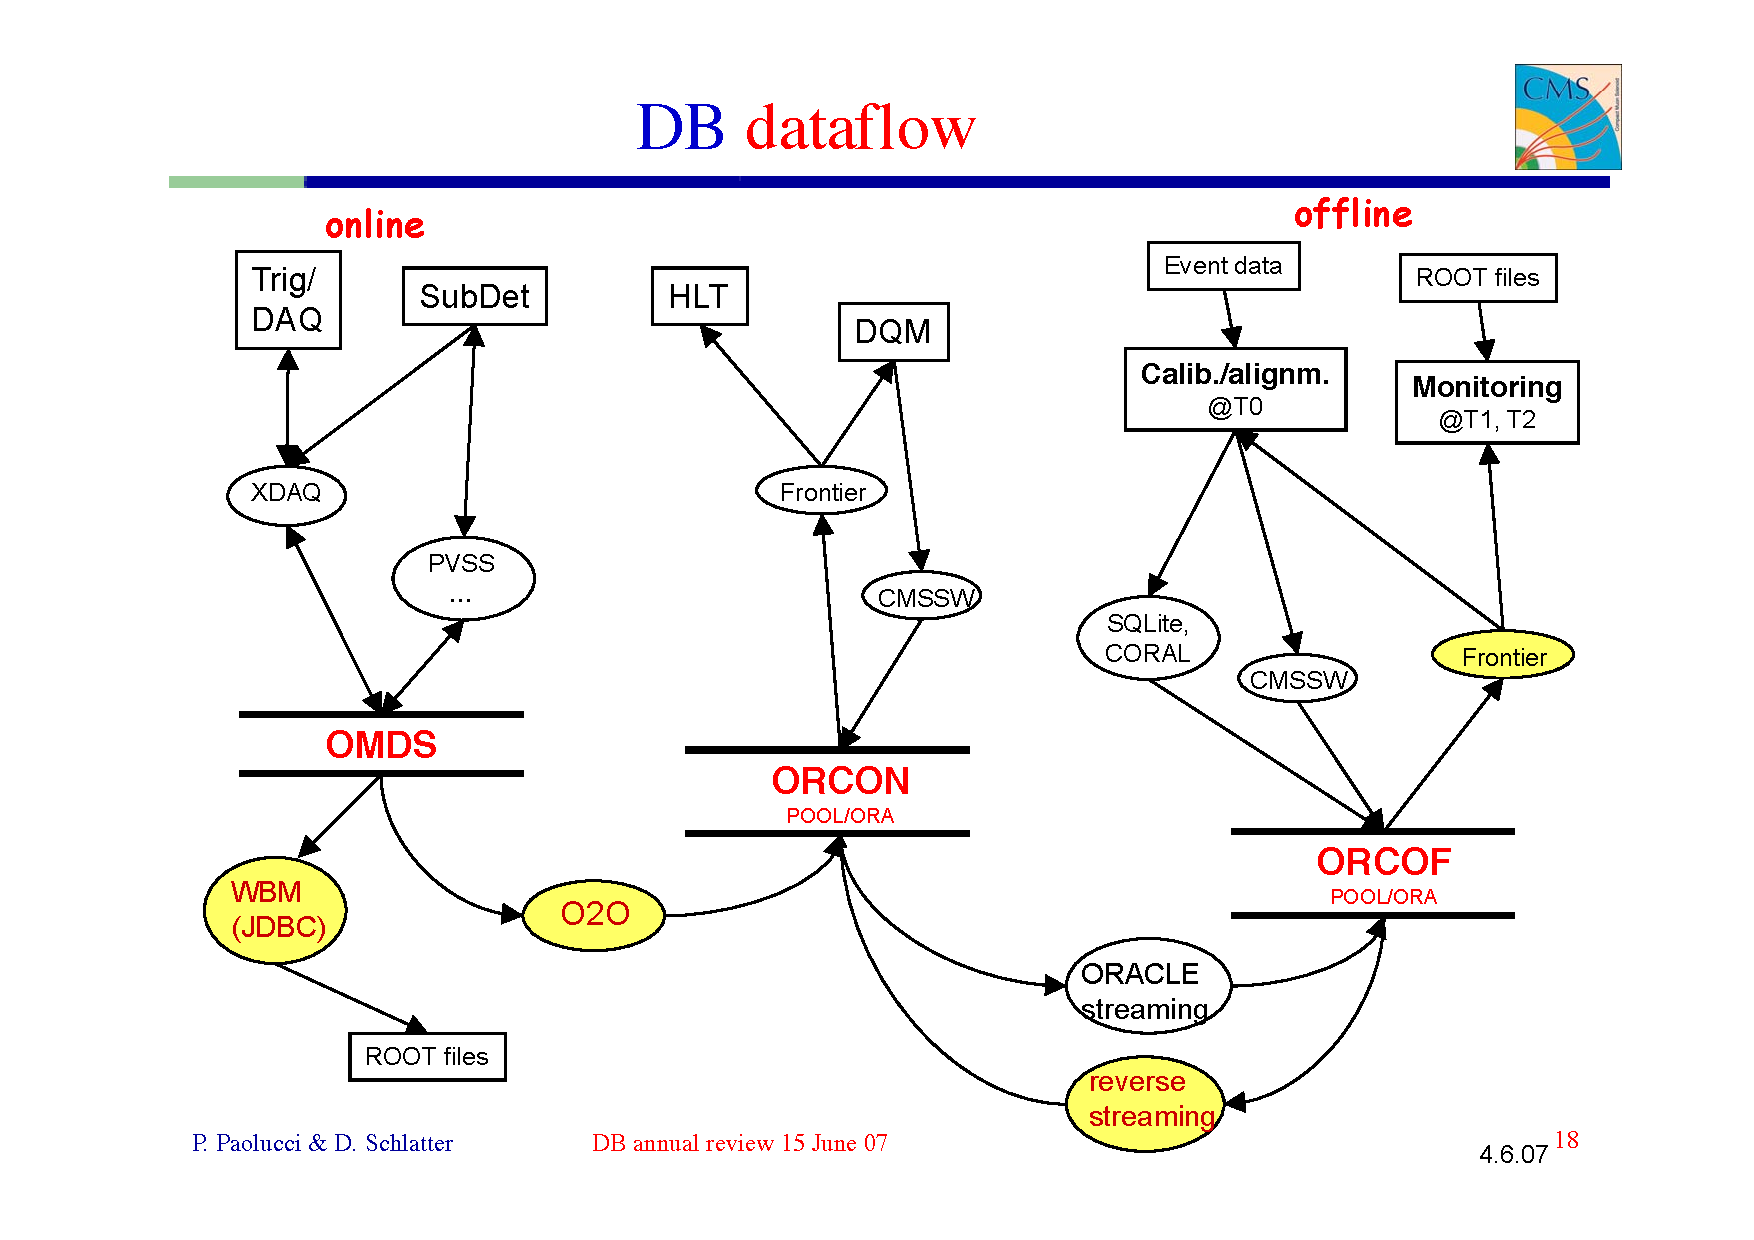
\includegraphics[width=0.9\textwidth]{DB}
\caption{Online Databases. Figure taken from \cite{talk:pigi}.}
\end{center}
\label{fig:database}
\end{figure}

% CHECK: some details in talks by 
%\bibitem{talk:giovanni} G.Franzoni,
%talk at DQM Workshop 27 August 2007,\\
%http://indico.cern.ch/conferenceDisplay.py?confId=19909
%\bibitem{talk:kcira} D.Kcira
%talk at weekly EvF/DQM meeting 31 May 2007,\\
%http://indico.cern.ch/conferenceDisplay.py?confId=15919\#6

\subsection{DAQ Monitor System}

The DAQ monitoring system XMAS provides access to live and persistent non-event 
(conditions) data describing the Detector hardware and readout system.
Work is ongoing to provide an interface which would allow that DQM applications 
can transparently receive online XMAS conditions data.
The near term goal is to create a DQM application which produces DQM histograms
containing distributions of DAQ system quantities.

\subsection{Computing Monitoring}

%=======================================================
% this subsection is common to all sections, please keep
\subsection{Integration and Support for Other Systems}

\subsubsection*{Integration}

\subsubsection*{Operation}


\section{DQM System Optimization}

\subsection{Core Software}
Core software components are largely in place now. 
In addition, experience with testing and operation within quasi-real production conditions
(e.g. CRUZET, CSA08) is bringing out a number of areas where
optimization is required in order to arrive at the design performance.

\subsection{Histograms, Alerts and Certification Algorithms}

This will be part of the DQM group's job:
\begin{itemize}
\item Standardization and refinement of DQM quality criteria.
\item Refinement of the selection of histograms relevant for online DQM.
\item Integration of validated source modules for operation in HLT.
\end{itemize}

\section{Summary}

\subsection{Technical Developments Summary}

A list of uncovered development issues is given in table \ref{tab:summary:devel}.

\begin{table}[h]
\begin{center}
\begin{tabular}{||l|l|l||}
\hline \hline
       & Description & FTE \\
       \hline
Online & Detector status, alarm and report & \\
       & summary logging to database & 1 month FTE \\
       & Commissioning of online DQM in HLT / run control & 3 months FTE \\
Offline & Scaling and production testing of harvesting step & \\ 
        & Integration of DQM task from Calibration and Alignment & \\ 
        & Layout of DQM at CAF & \\ 
Certification & Development of data certification framework code, & \\ 
         & i.e. read and combine DCS, DAQ and DQM info, & \\
	 & write output to DBS and condDB & 2 FTE for 4 months \\
GUI &  & \\
Core &  & \\
\hline \hline
\end{tabular}
\end{center}
\label{tab:summary:devel}
\caption{List of presently not sufficiently covered development projects with high priority}
\end{table}

\subsection{DQM System Integration and Operation Summary}

A list of integration, operation and maintenance tasks is given in table \ref{tab:summary:operation}.
Details can be found in the respective sections above.

\begin{table}[h]
\begin{center}
\begin{tabular}{||l|l|l||}
\hline \hline
       & Description & FTE \\
       \hline 
Core   &  Maintenance and Release Coordination  &
          for DQM, DQMOffline, Validation \\
       &  Subsystem support and code reviews \\
Online &  System operation and maintenance & \\
       &  24/7 on-call expert coverage & \\
       &  shifter instructions and supervision & \\
       &  documentation & \\
Offline &  & \\
Certification &  & \\
GUI &  & \\
Core &  & \\
\hline \hline
\end{tabular}
\end{center}
\label{tab:summary:operation}
\caption{List of Uncovered Development and Operation Tasks}
\end{table}


\begin{thebibliography}{99}

\bibitem{workshop070827} DQM Workshop 27 August 2007
\bibitem{webtools} CMS Data Management Webtools https://twiki.cern.ch/twiki/bin/view/CMS/DMWebtools
\bibitem{iguana} G.Eulisse, https://twiki.cern.ch/twiki/bin/view/CMS/CMSSW\_dqmIGUANAGUI
\bibitem{guimeeting} D.Menasce, L.Tuura, S.Dutta, P.Merkel, Private
communication
\bibitem{talk:lassi} L.Tuura, talk at weekly EvF/DQM meeting, 7 June 2007
http://indico.cern.ch/getFile.py/\\
access?contribId=29\&sessionId=6\&resId=0\&materialId=slides\&confId=16991
\bibitem{dqmbrowser} http://cmsmon.cern.ch/cmsdb/servlet/DQMBrowser?RUN=$<$runnumber$>$
\bibitem{talk:pigi} P.Paolucci,
talk at CMS annual review 15 June 07,
http://indico.cern.ch/getFile.py/\\
access?contribId=28\&resId=1\&materialId=slides\&confId=16736
\bibitem{talk:harry} H.Cheung, 
talk at DQM Workshop 27 August 2007, \\
http://indico.cern.ch/conferenceDisplay.py?confId=19909
\bibitem{datacert:gutsche} 
   http://indico.cern.ch/getFile.py/access?contribId=48\&sessionId=21\&resId=0\&materialId=slides\&c
onfId=28445   
\bibitem{datacert:meyer}   
   http://indico.cern.ch/getFile.py/access?resId=0\&materialId=slides\&contribId=44\&sessionId=21\&s
ubContId=1\&confId=28445

\end{thebibliography}
\end{document}



%%% Notes
%    +developments     
%     + core: timescale for baseline DQM
%       - history plots
%       - geometric navigation
%       - HIER NOCH MEHR PUNKTE EINFUEGEN
%       - make DQM software exportable, e.g. to Tier-1 and 2
%     + finish development and implementation of DQM file archival system
%       (online and offline).
%     + core: write summary online DQM information to conditions DB
%     + core: organize forwarding of relevant DB information from 
%       omds/orcon to orcoff
%     + core: set up framework for retrieval, calculation 
%       and writing of data certification info
%     + algorithms to be implemented by subsystems
%     
%     +technical developments and extension of DQM GUI and parts of framework 
%      for
%      + DAQ
%      + DB
%    +deployment
%     + implementation/use of HLTconfDB for DQM
%     + deployment of HLT DQM
%     + consolidation / run control integration of DQM off SM
%     + production testing of offline DQM at Tier-0
%     + implementation/support for AlcaReco Workflows
%     + validation of CSA08
%    +operation
%     + P5 (2 FTE for remaining developments, consolidation, on-call support)
%     + Tier-0
%     + support for CAF
%    +communication/documentation/user support/planning
